Thinking...
We need to translate Japanese sentences to English, preserving TeX code unchanged. The given text includes a figure environment with caption and label, and table entries with Japanese. Need to translate Japanese parts: the caption and the two table cell labels. Also maybe "高被引用論文全体" and "オブソレッセンス状態にある論文のみ". Also "高被引用論文のオブソレッセンスにかかる各指標値". Provide English translation while leaving TeX code unchanged.

Thus output should be the same TeX code but Japanese replaced by English.

So:

\begin{figure*}[h]
\begin{center}
{\small
\begin{tabular}{cc}
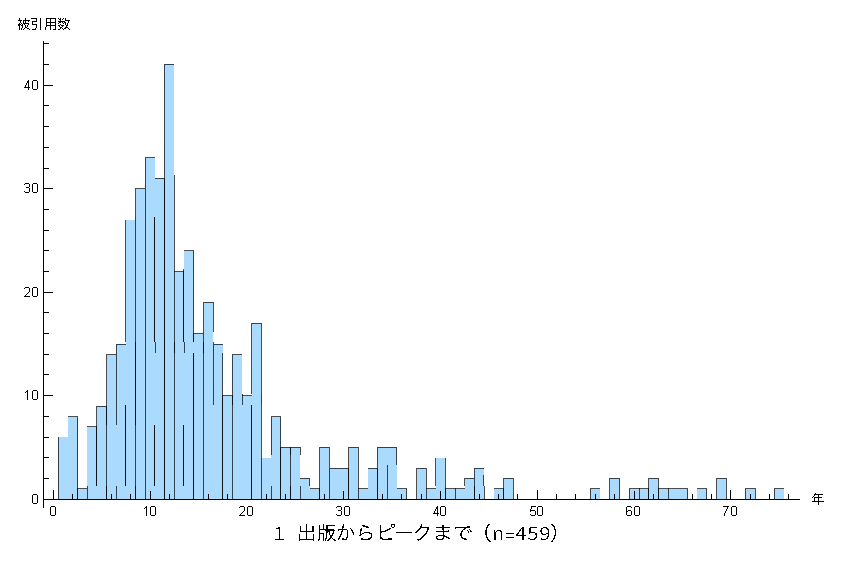
\includegraphics[width=75mm]{obsindex1-1.eps} & 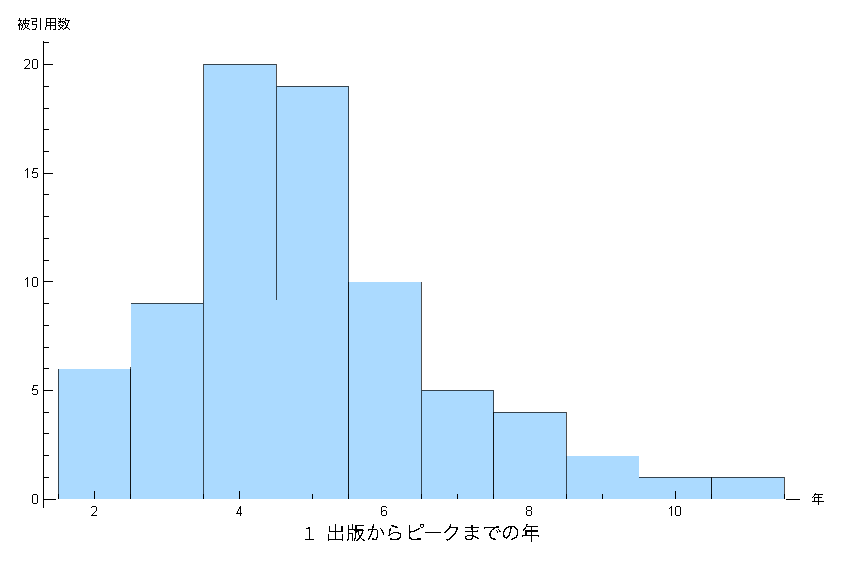
\includegraphics[width=75mm]{obsindex2-1.eps} \\
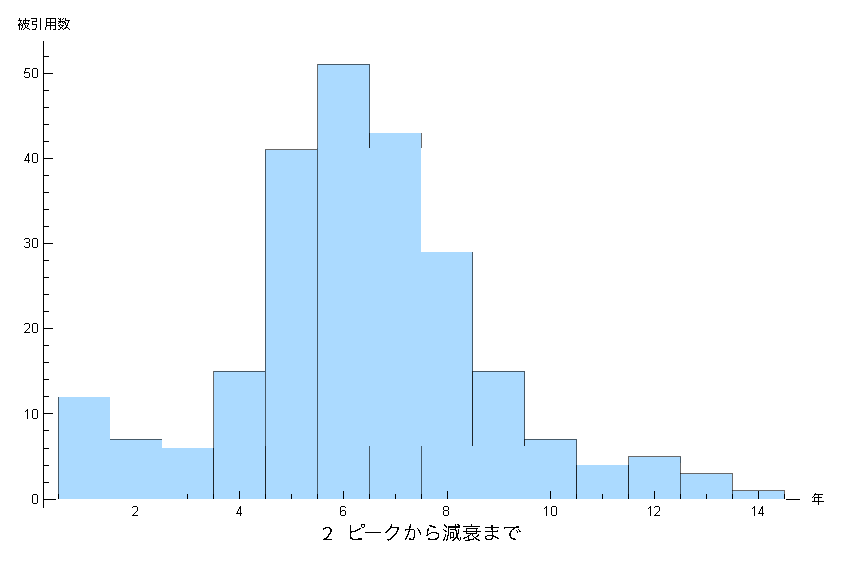
\includegraphics[width=75mm]{obsindex1-2.eps} & 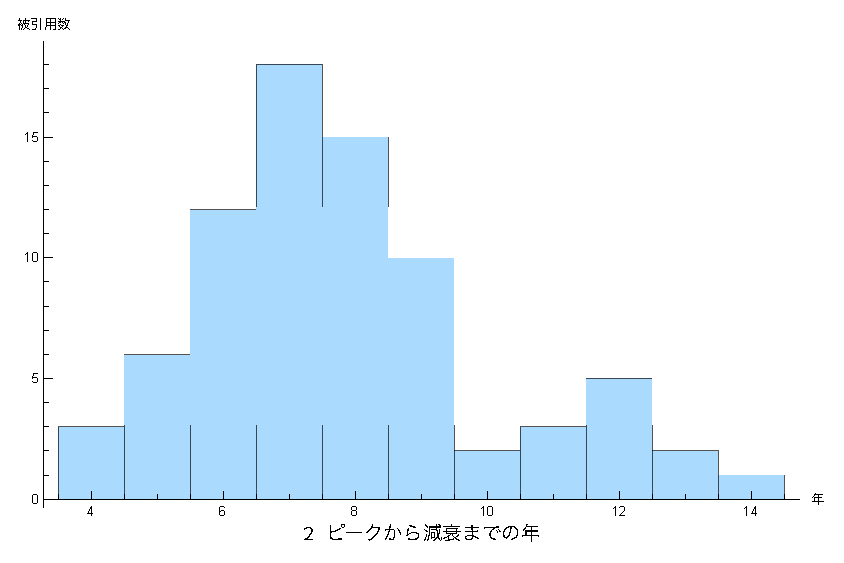
\includegraphics[width=75mm]{obsindex2-2.eps} \\
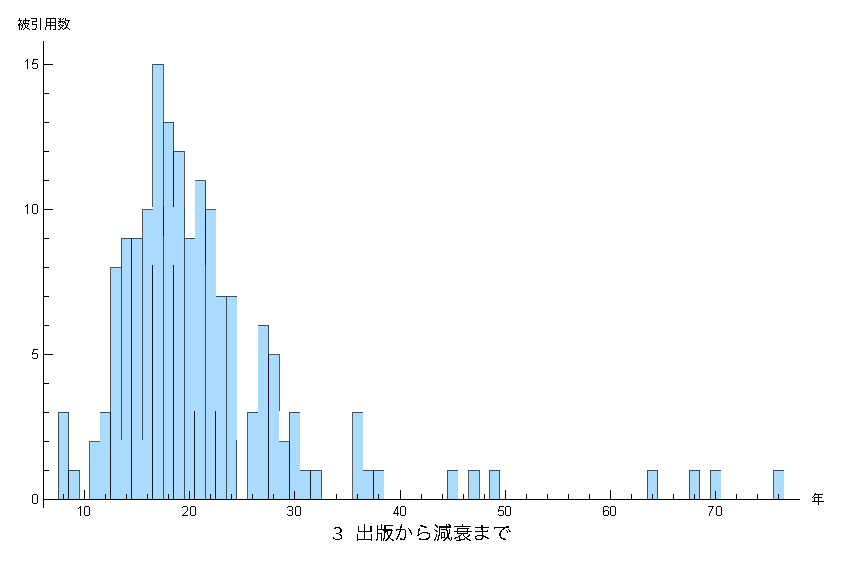
\includegraphics[width=75mm]{obsindex1-3.eps} & 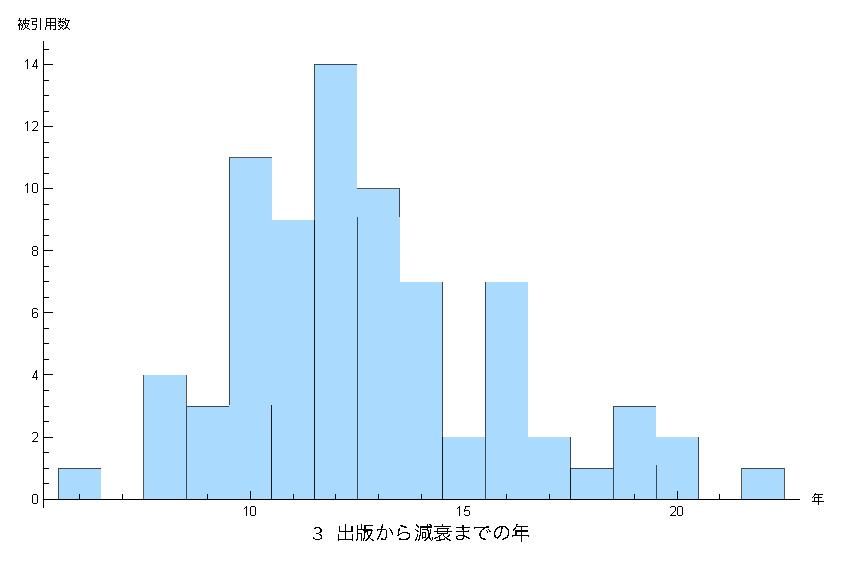
\includegraphics[width=75mm]{obsindex2-3.eps} \\
{\begin{tabular}{c}1. All highly cited papers\end{tabular}} & {\begin{tabular}{c}2. Only papers in an obsolescence state\end{tabular}} \\
\end{tabular}
}
\caption{Various metric values concerning the obsolescence of highly cited papers}
\label{fig:arr1}
\end{center}
\end{figure*}

Make sure the English translation is accurate. "高被引用論文全体" -> "All highly cited papers". "オブソレッセンス状態にある論文のみ" -> "Only papers that are in an obsolescence state". Caption: "各指標値" means "each metric values". So "Metric values related to the obsolescence of highly cited papers". Could be "Metric values concerning the obsolescence of highly cited papers". Good.

Return only the translated LaTeX block.

...done thinking.

\begin{figure*}[h]
\begin{center}
{\small
\begin{tabular}{cc}
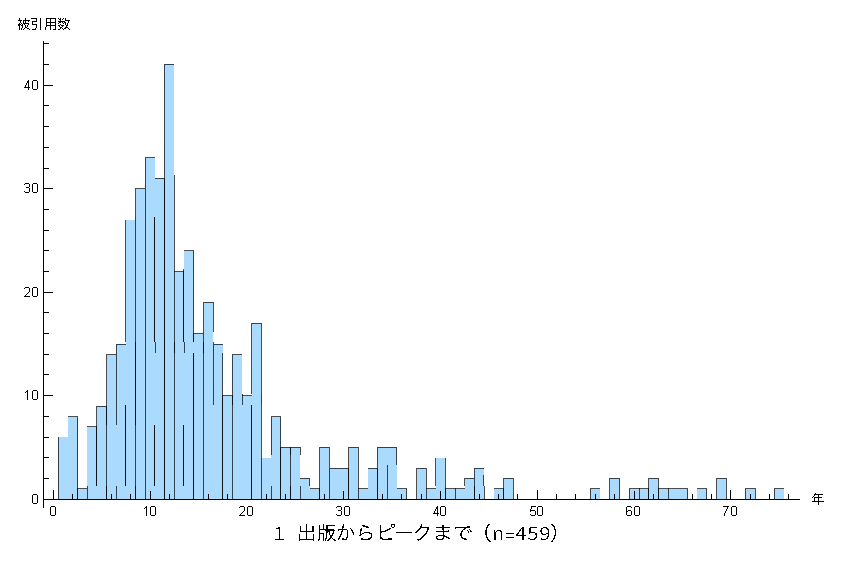
\includegraphics[width=75mm]{obsindex1-1.eps} & 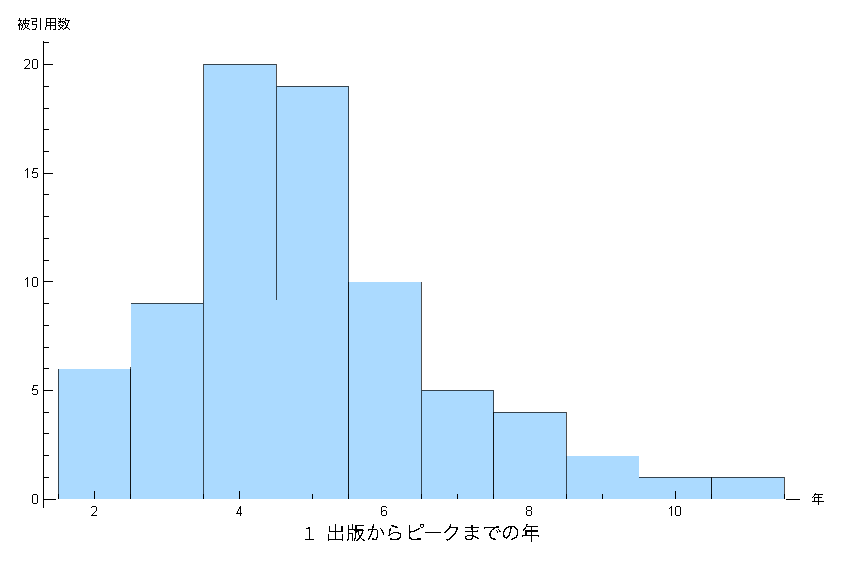
\includegraphics[width=75mm]{obsindex2-1.eps} \\
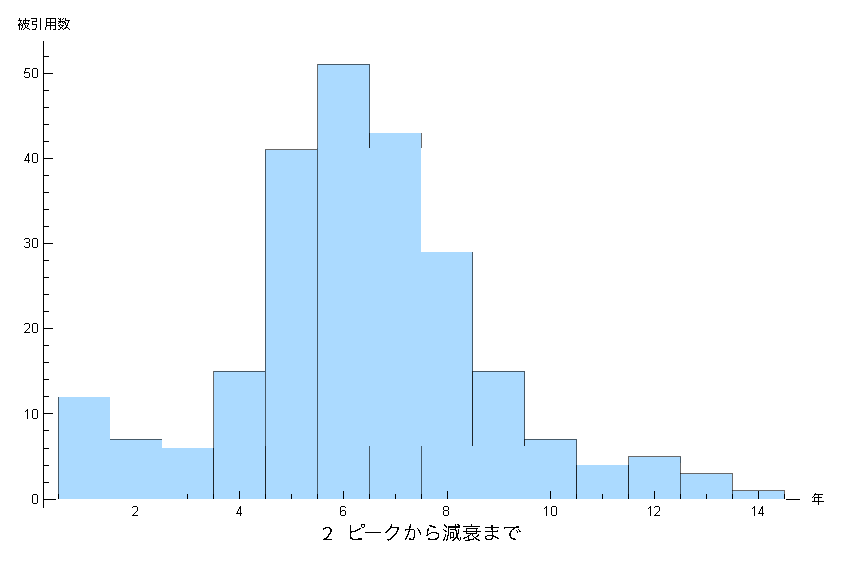
\includegraphics[width=75mm]{obsindex1-2.eps} & 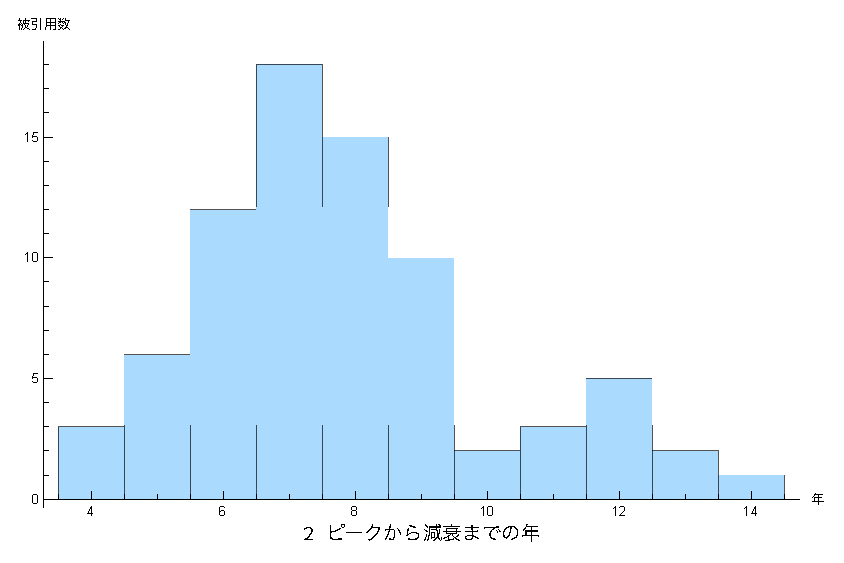
\includegraphics[width=75mm]{obsindex2-2.eps} \\
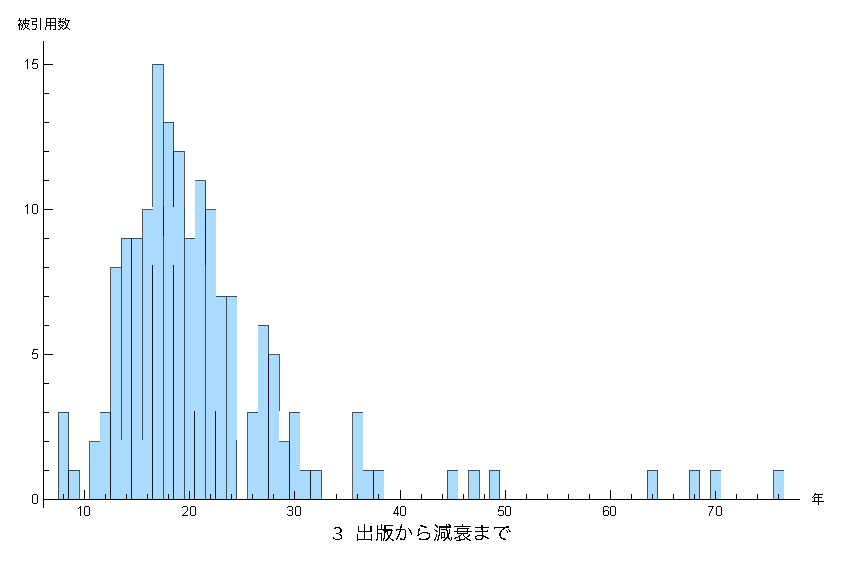
\includegraphics[width=75mm]{obsindex1-3.eps} & 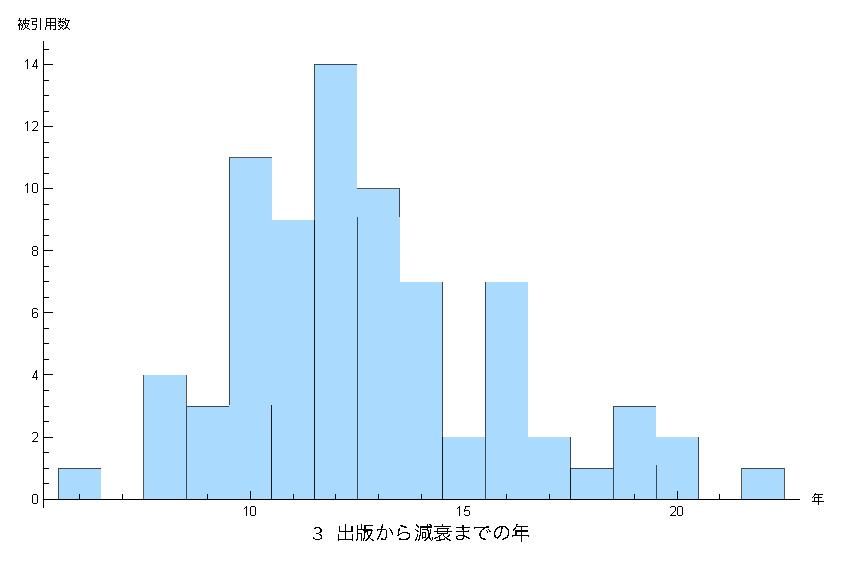
\includegraphics[width=75mm]{obsindex2-3.eps} \\
{\begin{tabular}{c}1. All highly cited papers\end{tabular}} &
{\begin{tabular}{c}2. Only papers in an obsolescence state\end{tabular}} \\
\end{tabular}
}
\caption{Metric values concerning the obsolescence of highly cited papers}
\label{fig:arr1}
\end{center}
\end{figure*}

